% mainfile: ../../../../master.tex
\subsection{DNA quantification with Qubit\texttrademark~ DNA BR Assay Kit}
% The part of the label after the colon must match the file name. Otherwise,
% conditional compilation based on task labels does NOT work.
\label{task:20180215_cj1}
\tags{lab,qnt,dna}
\authors{cj}
%\files{}
%\persons{}

Just to make sure the results are robust, I quantify twice the same sample using two different volumes: 5~\uL and 10~\uL. Based on these two measurments and calculation, I can be pretty sure of the actual concentration of my sample. 

And to assess the reproducibility of the measurments, I just measure twice the same samples (I also repeat the calibration).

\begin{figure}[H] % position of the figure 
    \centering
    \caption{Illustration for the Qubit\texttrademark~ DNA BR assay}
    \label{fig:20180215_Qubit_dsDNA_BR}
    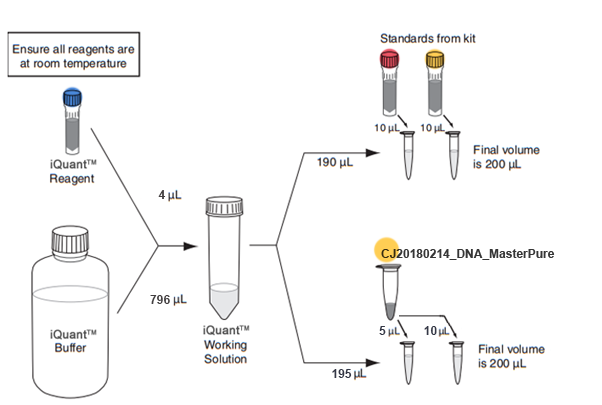
\includegraphics[width=0.8\textwidth]{graphics/schemas/20180215_Qubit_dsDNA_BR.png}
\end{figure}

In table \ref{tab:20180215_nuc_acid_qnt}, the quantities of DNA are calculted based on the volume left: I know I resuspended my DNA pellet in 50~\uL of Tris HCl buffer, then I used 2~\uL for the NanoDrop\cR measurments and finally I use 5~\uL and 10~\uL for the Qubit\texttrademark~ assay. Which means the volume left us 33~\uL. But based on these results, the original amount of DNA I was able to retrieve is -- at least -- 0.910 ng, which is almost 1~\textmu g of DNA!

\begin{table}[H]
\caption{Total DNA quantities in samples measured with Qubit\texttrademark~ DNA BR Assay Kit}
\label{tab:20180215_nuc_acid_qnt}
\centering
\begin{tabular}{l r r r r}
\toprule
Sample ID & \textmu g/mL & $V_f$ (mL) & m (\textmu g) & m (ng) \\ \midrule
\texttt{CJ20180214\_DNA\_MasterPure\_5} & 20.0 & 0.033 & 0.66 &  660.00 \\
\texttt{CJ20180214\_DNA\_MasterPure\_10} & 18.5 & 0.033 & 0.610 & 610.50 \\
\texttt{CJ20180214\_DNA\_MasterPure\_5} & 20.1 & 0.033 & 0.663 & 663.30 \\
\texttt{CJ20180214\_DNA\_MasterPure\_10} & 18.2 & 0.033 & 0.600 & 600.60 \\
\bottomrule
\end{tabular}
\end{table}


